\chapter{Spatial and temporal relationships between GTHA data sources} \label{ch:spatial_and_temporal_relationships_between_urban_data}

\section{Chapter 3: data sources used in the GTHA housing market database} \label{sec:chapter_3_intro}
%TODO rewrite intro about spatial and temporal relationships (was data sources before)
Most urban areas are divided into zones or planning areas on the basis of maintaining similar population sizes and following built or natural boundaries like roads or rivers.
To simulate the changes in accessibility, metropolitan regions are usually broken down into a set of small geographic zones, similar (or in many cases identical) to the set of zones used for regional travel forecasting.
Changes to relative accessibility of a location can thus be estimated as changes in zone-to-zone travel times in a travel network\cite{Iacono2008}.


The proposed GTHA housing market database combines urban data coming from a variety of sources.
At the heart of it lies Teranet's dataset of real estate transactions (land registration records) recorded in the Province of Ontario since the beginning of XIX century up to October of 2017.
As was discussed in section~\ref{subsec:challenges_quality_skills_features}, one of the main challenges of working with Teranet's data is the lack of available features.
At the same time, Teranet records have timestamps (dates) and location information (x and y coordinates) and thus can be joined to variety of other urban data sources, such as Census demographics, Transportation Tomorrow Survey (TTS) and parcel-level land use information.

However, as will be discussed in this chapter, these data sources use different spatial units and are available at different temporal spans.
Therefore, when joining data from these sources, special consideration needs to be taken with respect to their temporal and spatial relationships to ensure semantic interoperability.
These spatial and temporal relationships are implemented via the data preparation workflow in Python and a PostgreSQL relational database, design and implementation of which is the primary focus of this master's thesis.

The nature of spatial and temporal relationships between the various data sources used in the proposed GTHA housing market database is discussed in this chapter, implementation of relationships is discussed in chapters~\ref{ch:data_preparation} and~\ref{ch:rdbms_design} of this master's thesis.

\subsection{Accessibility as a measure of land use-transportation relationship} \label{subsec:accessibility}

While transportation research started as an isolated field focusing on mobility, researchers recognized that trips are made to access particular destinations\cite{VanLierop2017}.
A concept of accessibility, understood as the ease of reaching rather than simply the ease of moving\cite{Preston2007}, was developed to take into account the location of urban opportunities.
Accessibility is the mediating factor between the location of activities and demand for travel and is discussed further in section~\ref{subsec:accessibility} of the following chapter.

LUT models (discussed in section~\ref{subsec:transportation_land_use_interaction}) operationalize the transportation-land use relationship by incorporating measures of accessibility with the process of locating activities, typically assuming that households wish to locate in areas with higher accessibility to employment, shopping, or entertainment opportunities.
Similarly, firms are assumed to locate in areas with higher accessibility to labour markets.
Land use component is usually integrated into the accessibility measure through congested network travel times.
However, when studying the relationship between transportation facilities and property values, results may vary based on whether travel time or travel distance is used as a measure of accessibility\cite{Sherry1999}.

Accessibility measures the situation of a location relative to other activities or opportunities (work, shopping, etc.) distributed in space and can be an important determinant of price in LUT models where land and floor space markets are considered explicitly\cite{Iacono2008}.
When measuring changes in relative accessibility, it is usually approximated by some measure of access to the transportation network, such as travel time or distance.

Economic decisions made by the households and firms act as one of the links between the tranportation and land use systems.
When choosing a location, households and firms attempt to fulfill as many of their location preferences as possible while facing constraints.
One of the main constraints is the price or rent of the dwelling, related to the income of the household;
another important constraint is travel time, with suitable location being restricted by the travel times and transportation expenses\cite{Moeckel2017}.

\section{Description of data sources} \label{sec:description_of_data_sources}

This section describes different data sources combined into the GTHA housing market database.

\subsection{List of data sources that are currently used in the database} \label{subsec:list_of_data_sources}

Currently, the following data sources are available in the GTHA housing market database:

\begin{enumerate}
    \item Teranet's dataset
    \begin{itemize}
        \item real estate transactions (land registration records) recorded in Ontario
    \end{itemize}
    \item Select variables, tables from Census of Canada
    \begin{itemize}
        \item demographics
        \item statistics
        \item Dissemination Area (DA) geometry
    \end{itemize}
    \item Select variables, tables from Transportation Tomorrow Survey (TTS)
    \begin{itemize}
        \item information about the transportation network
        \item Transportation Analysis Zones (TAZ) geometry
    \end{itemize}
    \item DMTI Spatial
    \begin{itemize}
        \item parcel-level land use by year (2001-2014)
        \item enhanced points of interest (EPOI) by year (2001-2013)
        \item postal geography
        \item FSA geometry
    \end{itemize}
    \item land use information from University of Toronto's Department of Geography
    \begin{itemize}
        \item detailed parcel-level land use information collected in 2011
    \end{itemize}
\end{enumerate}

Different data sources and their spatial and temporal relationships are discussed in the remainder of this chapter.

\subsection{Teranet's dataset of land registration records} \label{subsec:teranet_description}

Teranet's dataset\cite{TeranetEnterprisesInc.2011} of real estate transactions (land registration records) recorded in the Province of Ontario holds a wealth of information on the housing market of Ontario.
Due to the introduction of POLARIS (discussed in section~\ref{subsec:polaris}) by the Province of Ontario in 1985, Teranet's dataset includes a complete population of real estate transactions recorded in Ontario from 1985 up to October of 2017 (records prior to 1985 appear to be incomplete, see chapter~\ref{ch:eda_results}).
Since Teranet's dataset has a high number of records, it can be used to investigate aspects relating to the housing market at a very fine spatial and temporal scale.

At the same time, Teranet's dataset is very limited on the amount of features available for each record.
Since each record has a timestamp and is geocoded, Teranet's dataset can be augmented by joining additional attributes from various data sources, such as Census or TTS survey, based on spatial and/or temporal relationships.

\vspace{5mm}

Characteristics of the raw Teranet dataset:
\begin{itemize}
    \item 9,039,241 rows
    \item 15 columns
\end{itemize}

Characteristics of the Teranet dataset after data preparation (described in chapter~\ref{ch:data_preparation}):
\begin{itemize}
    \item 5,188,513 rows
    \item 75 columns
\end{itemize}

Every record in Teranet's dataset is geocoded with a pair of coordinates (latitude and longitude).
These coordinates are supposed to represent the centroid of the corresponding parcel, but might not always be that accurate.

\subsection{Census of Canada} \label{subsec:census_description}

One of the major sources of demographic and statistical data in Canada are the datasets collected under the national Census program.
Census data provide valuable insight into the latest economic, social and demographic conditions and trends in Canada and is used to plan important public services.
Statistics Canada collects every five years the national Census of Canada and disseminates the information by a range of geographic units, also referred to as "Census geography"\cite{MapandDataLibrary2019}.

Census geography follows a certain hierarchy defined by Statistics Canada, with the largest top-level divisions being provinces and territories, lowest-tier divisions to which census data is disseminated are Dissemination Areas (DAs)\cite{StatisticsCanada2018}.
Statistics Canada defines a dissemination area as a small area composed of one or more neighbouring dissemination blocks, roughly uniform in population size targeted from 400 to 700 persons to avoid data suppression\cite{StatisticsCanada2015}.

\subsection{Transportation Tomorrow Survey (TTS)} \label{subsec:tts_description}

Another major source of information for most transportation planning studies concerned with Southern Ontario is the Transportation Tomorrow Survey (TTS)\cite{DataManagementGroup2014}, an origin-destination travel survey.
The Transportation Tomorrow Survey (TTS), undertaken every five years since 1986, is a cooperative effort by local and provincial government agencies to collect information about urban travel in southern Ontario.

TTS represents a retrospective survey of travel taken by every member (age 11 or over) of the household during the day previous to the telephone or web contact.
The information collected and the method of collection has remained relatively consistent over the seven surveys and includes characteristics of the household, characteristics of each person in the household, and details of the trips taken by each member of the household, including details on any trips taken by transit\cite{Ashby2018}.

The finest level of spatial aggregation is that of the Traffic Zone also referred to as Traffic Analysis Zone (TAZ).
The Traffic Zone is a polygon which typically falls along the centre line of roads or the natural geographic boundaries\cite{DataManagementGroup2019}.
Not as a rule, but the TAZs roughly follow census tract boundaries, which are slightly bigger than DA boundaries.

TTS data has been collected for changing TAZ boundaries or in other words, different zone systems due to growing population and expanding extents of the survey in the GTHA region over the years.
To make the TTS data consistent for comparing over all years from 1986 to 2016, the Data Management Group (DMG), the custodian of the dataset derived from TTS, made all surveys available in the 2001 zone system, for convenience of researchers (any zone system could have been chosen for that matter).

UTTRI used the 2001 TAZ system to model travel times for the GTHA on EMME for all TTS years based on the origin-destination trip data collected in the survey.
The travel time data was used to create further transportation accessibility variables.

\subsection{DMTI data} \label{subsec:dmti_data}

DMTI Spatial, a Digital Map Products company, is a major provider of location based information in Canada.
DMTI's Enhanced Points of Interest (EPOI) is a vector GIS database of over 1 million business and recreational points of interest for all provinces/ territories of Canada.
The attribute information contains multiple feature types and categories, information is available by year.
Spatial units used by DMTI datasets used in the GTHA housing market database are points and parcel polygons, available by year.

\subsection{Detailed land use information from geography department} \label{subsec:detailed_land_use_from_geogrpahy_department}

The detailed land-use data collected by University of Toronto's Department of Geography is a combination of parcel boundaries (from Teranet) and manually coded land-use data using Google maps and streetviews, provided by Prof.
Andre Sorensen and Prof.
Paul Hess's research project.
The spatial unit used by land use data provided by the Department of Geography is a parcel polygon.

\section{Spatial relationships between datasets} \label{sec:spatial_relationships}

%TODO finish section
This section introduces the spatial relationships between the datasets used in the GTHA housing market database.


\subsection{Spatial units used by the data sources in the GTHA housing market database} \label{subsec:spatial_units_used_in_database}

The following spatial units are being used by different sources in the GTHA housing market database:

\begin{itemize}
    \item Point data
    \begin{itemize}
        \item Teranet
        \item EPOI from DMTI
    \end{itemize}
    \item Parcel-level data (polygons)
    \begin{itemize}
        \item detailed land use from the Department of Geography
        \item land use from DMTI
    \end{itemize}
    \item DA-level data (polygons)
    \begin{itemize}
        \item Census variables
    \end{itemize}
    \item TAZ-level data
    \begin{itemize}
        \item TTS variables
    \end{itemize}
\end{itemize}

%TODO write about the challenge of joining polygons

\section{Temporal relationships between datasets} \label{sec:termporal_relationships_between_datasets}

\subsection{Temporal spans at which different urban data sources are available} \label{subsec:temporal_scales}

%TODO write a section about temporal scales
Figure~\ref{fig:temporal_spans} presents temporal spans of the data sources used in the GTHA housing market database.
\begin{figure}[hbt!]
    \centering
    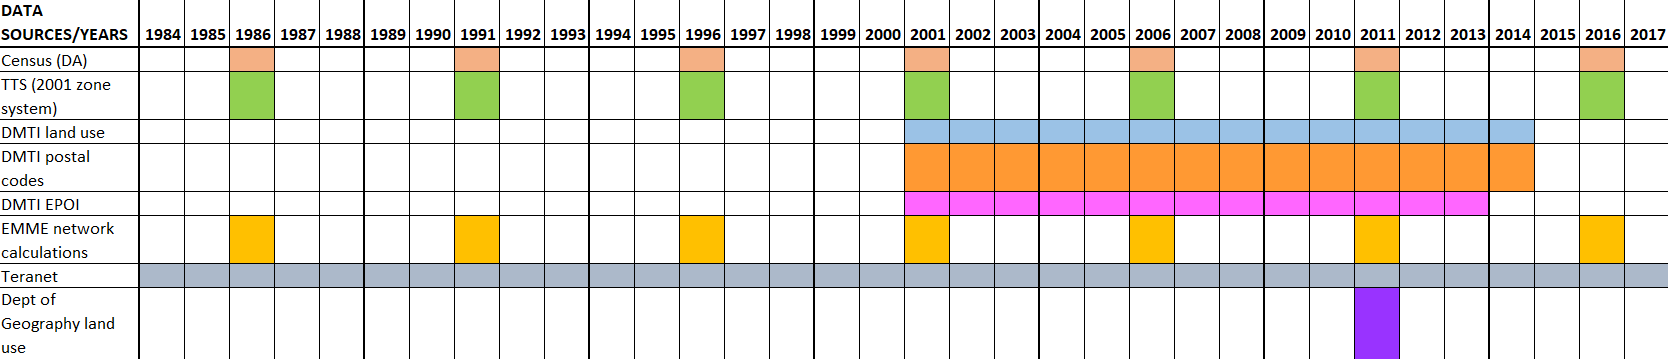
\includegraphics[width=1\linewidth,trim=0 0 0 0,clip]{temporal_spans.png}
    \caption{Temporal spans of the data sources used in the GTHA housing market database.}
    \label{fig:temporal_spans}
\end{figure}

\subsection{Possible approaches to matching temporal spans to relate data sources} \label{subsec:possible_approaches_to_match_temporal_spans}

Teranet and Census / TTS variables can be matched in a number of ways:

\begin{enumerate}
    \item Direct match with appropriate Teranet subsets
    \begin{itemize}
        \item use subsets of Teranet records from the Census / TTS years and match only with data directly recorded for that year
        \item for example, take a subset of Teranet records from 2016 and match it with 2016 Census / TTS variables
        \item technically, any date span can be specified when creating a Teranet subset, but in this case, appropriate Census / TTS variables must be selected manually
        \item benefits:
        \begin{itemize}
            \item precision of match: variables from Census would be composed of the actual values produced by the survey, rather than an interpolation based on assumptions
            \item flexibility of use: a new Census table can be added and its variables can be match with appropriate Teranet records via simple SQL queries
        \end{itemize}
        \item disadvantages:
        \begin{itemize}
            \item limited match: only Teranet data from Census years can be used, records from between Census years cannot be matched with the Census vairables
            \item hard to generalize SQL queries: need custom SQL queries to match data to different tables, several queries to match Teranet data from different Census years
        \end{itemize}
    \end{itemize}
    \item Interpolation of discrete Census / TTS variables
    \begin{itemize}
        \item discrete Census / TTS variables can be turned into continuous via interpolation
        \item Teranet records can be matched to real recorded and interpolated values by year, or finer time scale
        \item benefits:
        \begin{itemize}
            \item most Teranet records used: all Teranet records within the Census / TTS range can be used (within the interpolation region)
            \item closest match: closest temporal match between Teranet records and Census / TTS variables
            \item precise, if correctly assessed: in the case where correct assumptions are made while interpolating values, the most precise match
        \end{itemize}
        \item disadvantages:
        \begin{itemize}
            \item more assumptions: additional assumptions need to be made about the dynamics of each Census / TTS variables between Census years
            \item inaccurate, if incorrectly assessed: in case of incorrect assumptions, there is a risk of lower accuracy compared with other matching methods
            \item interpolated rather then recorded: Teranet values from non-Census years will be matched to variables that are interpolated rather then recorded
            \item more data pre-processing needed: each Census / TTS variable needs to be processed in order to produce interpolated values
        \end{itemize}
    \end{itemize}
    \item Assign temporal spans for each Census / TTS survey as new features to Teranet records
    \begin{itemize}
        \item each Census / TTS survey can be assigned a temporal span of 5 years representing a group of Teranet records to which its variables can be matched
        \item Teranet records are matched by year, each year would yield an appropriate Census or TTS variable from an appropriate temporal span
        \item for example, the Census of 2016 would have a temporal span of 2014--2018, and thus a Teranet record from 2015 would be matched to variables from 2016 Census.
        \item Census of 1991 would have a temporal span of 1989--1993, and thus a Teranet record from 1993 would be matched with variables from 1991 Census.
        \item TTS survey would be matched in a similar manner
        \item benefits:
        \begin{itemize}
            \item most Teranet records used: all Teranet / TTS records that fall within the specified temporal spans range can be matched to appropriate Census / TTS variables
            \item recorded rather than interpolated: Teranet records are matched to actual recorded Census / TTS values
            \item avoid interpolation assumptions: since no interpolation is performed, no additional assumptions are needed
            \item no additional data pre-processing: all matching is done through an "adapter" table, original Census / TTS variables do not need to be changed
        \end{itemize}
        \item disadvantages:
        \begin{itemize}
            \item step-change in Census / TTS variables: when matching Teranet sources from non-Census years, instead of using interpolation, same Census / TTS variables are used for a group of 5 years centered at each Census year
            \item varying accuracy: accuracy of match further away from the Census years (+/- 2 years) probably will be lower.
            In addition, there would be a step change from every +2 to -2 Census year (i.e., 1998 to 1999)
            \item need new foreign keys: additional features specifying the temporal spans of Census / TTS variables to years for each Teranet record needs to be added to the Teranet table to facilitate temporal integrity of the joining operations
            \item Census and TTS tables need to be in a "tidy" data format, with each variable being a column, and each observation being a row.
            Year of Census and TTS needs to be encoded as a separate variable `year`, `year` and `dauid` or `taz\_o` becoming the primary keys of TTS and Census tables.
            In a case of a large number of variables such transformation makes Census table "long" instead of "wide".
        \end{itemize}
    \end{itemize}
\end{enumerate}


\subsection{Matching temporal scales to facilitate linking datasets} \label{subsec:matching_temporal_scales}
%TODO write a subsection about matching temporal scales

\section{Chapter summary} \label{sec:data_sources_summary}
Different data sources use different spatial and temporal scales, and that's what we are going to address with data prep and the database.
%TODO write chapter summary
